\documentclass[11pt,a4paper]{article}
\usepackage[T1]{fontenc}
\usepackage[english]{babel}
\usepackage{lmodern}
\usepackage[margin=2cm,top=2.1cm,bottom=2cm]{geometry}
\usepackage{amsmath,amssymb,graphicx,booktabs,tabularx,array}
\usepackage{microtype,fancyhdr,caption}
\usepackage[hidelinks]{hyperref}
\hypersetup{pdftitle={GPU Computing -- Exercise 2 -- Group 15},
  pdfauthor={Michele Arrigoni, Francesco Foresti, Kasra Ghasemipoo, Karol Bonat}}

\graphicspath{{figures/}{../raw/template/figures/}}
\setlength{\parindent}{0pt}
\setlength{\parskip}{0.45em}
\setlength{\emergencystretch}{2em}
\setlength{\headheight}{14pt}
\setlength{\tabcolsep}{8pt}
\renewcommand{\arraystretch}{1.12}
\captionsetup{font=small,labelfont=bf,skip=6pt}
\pagestyle{fancy}
\fancyhf{}
\fancyhead[L]{\small GPU Computing -- Exercise 2}
\fancyhead[R]{\small Group 15}
\fancyfoot[C]{\thepage}
\renewcommand{\headrulewidth}{0.3pt}
\newcommand{\us}{\,\mu\mathrm{s}}
\newcommand{\code}[1]{\texttt{#1}}

\begin{document}

\begin{center}
{\LARGE\bfseries GPU Computing -- Exercise 2}\par
\vspace{0.4em}
Heidelberg University -- Winter Term 2026/2027\par
\vspace{0.5em}
\textbf{Group 15}\par
Michele Arrigoni, Francesco Foresti, Kasra Ghasemipoo, Karol Bonat
\end{center}

We measured the overhead of launching CUDA kernels, the amount of work needed
to hide that overhead, and the bandwidth of transfers between host and device
memory. The report uses the four completed jobs listed below. The PCIe run
reports an NVIDIA GeForce RTX 2080 Ti; the logs do not record compiler versions
or compute-node names for these executions.

\begin{center}
\small
\begin{tabularx}{\linewidth}{@{}X r l@{}}
\toprule
Experiment & Job & Repetitions \\
\midrule
2.1: baseline comparison & 279658 & 100000 per mode \\
2.1: configuration sweep & 279659 & 1000 per mode and configuration \\
2.2: break-even search & 279660 & 100000 per wait duration \\
2.3: PCIe transfers & 279661 & 4--1000 per condition \\
\bottomrule
\end{tabularx}
\end{center}

\section*{2.1 Raw Kernel Startup Time}

\subsection*{Baseline comparison}
We started with an empty kernel launched with one block and one thread. In the
asynchronous test, we issued all launches and called
\code{cudaDeviceSynchronize()} once at the end. In the synchronous test, we
called it after every launch. The host timer measures the total elapsed time
\(\Delta t\); the mean time per launch is
\[
    \overline{t}=\frac{\Delta t}{N},\qquad N=100000.
\]

\begin{center}
\begin{tabular}{@{}lr@{}}
\toprule
Mode & Mean time (\(\mu\mathrm{s}\)) \\
\midrule
Asynchronous batch & 5.55 \\
Synchronization after every launch & 6.04 \\
\bottomrule
\end{tabular}
\end{center}

The synchronous mean is about \(8.8\%\) higher in this run. There is an
important detail in this comparison: the baseline program does not warm up
CUDA before starting its first timer. Its asynchronous result can therefore
include initialization costs, spread over the batch. This is a likely reason
why it is higher than the warmed-up asynchronous times in the configuration
sweep.

These values include submitting the work and waiting for the whole test to
finish. They are not measurements of the empty kernel's device execution time
alone. In particular, the asynchronous test measures the rate at which a
completed batch can be processed; it does not time an isolated host API call.
Kernel launches themselves are asynchronous with respect to the host.

\clearpage
\subsection*{Varying the launch configuration}

We tested the following numbers of blocks and threads per block:
\[
\begin{aligned}
    n_b &= 2^i, & i&=0,\ldots,14,\\
    n_t &= 2^j, & j&=0,\ldots,10.
\end{aligned}
\]
This gives \(15\times11=165\) configurations, from 1 to 16384 blocks and from
1 to 1024 threads per block. Before measuring each configuration, we ran one
untimed kernel and synchronized. We then timed 1000 launches in each mode and
divided the elapsed time by 1000.

\begin{figure}[!ht]
\centering
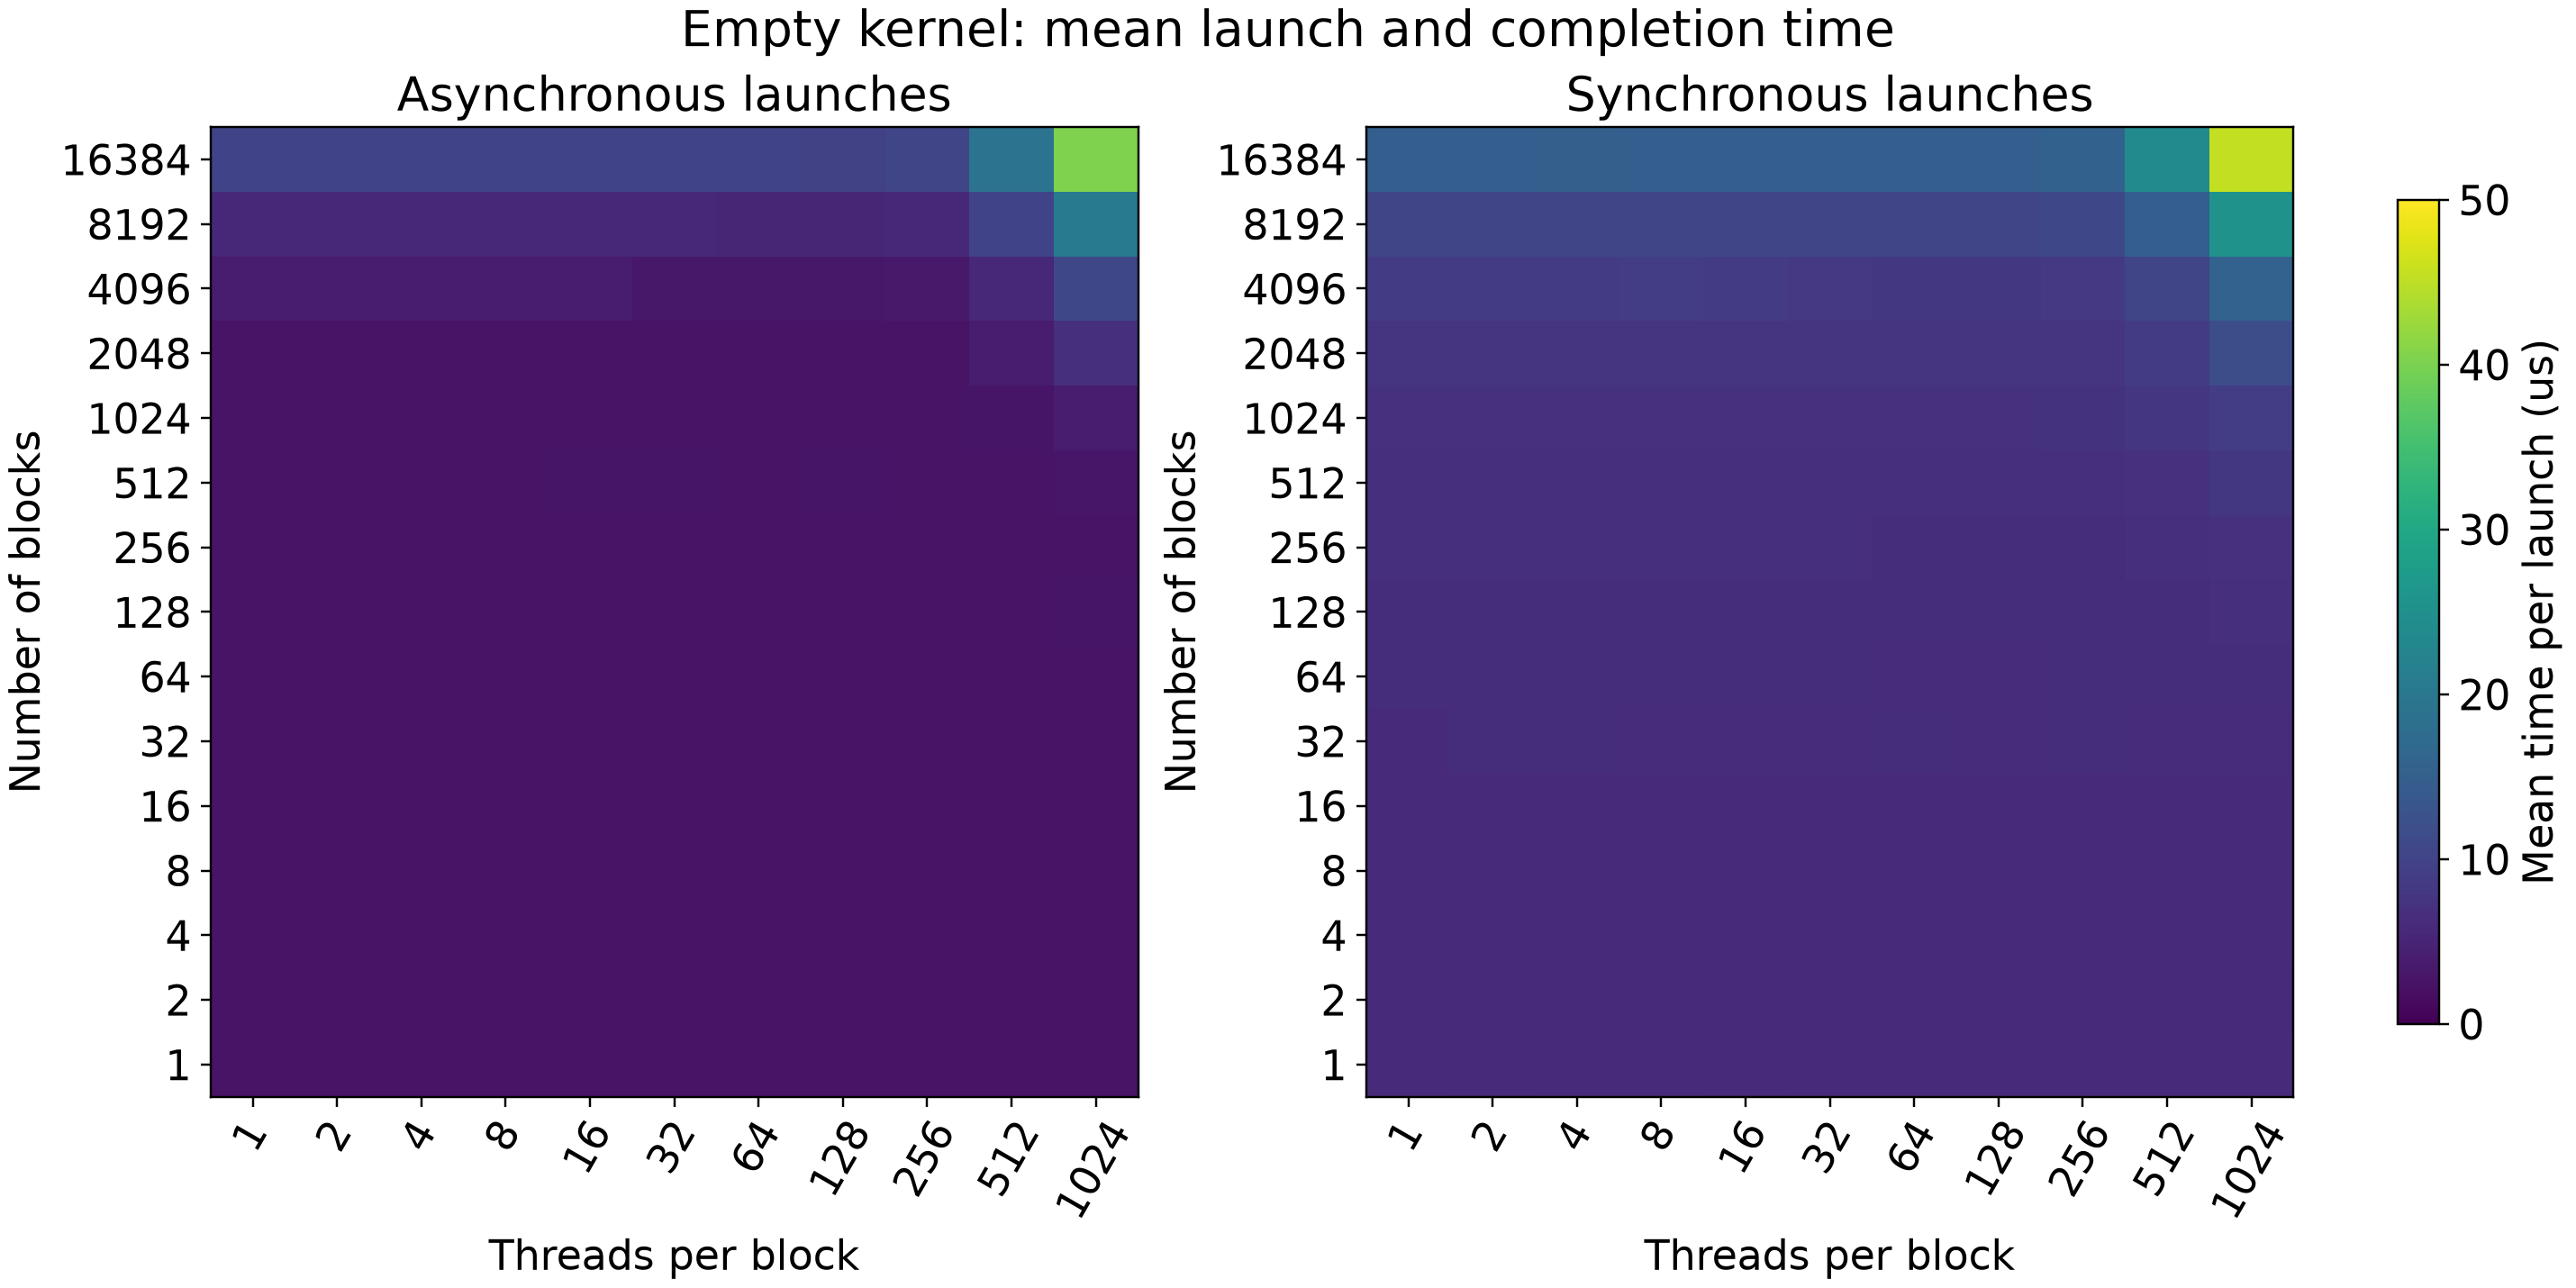
\includegraphics[width=\linewidth]{launch_heatmaps.png}
\caption{Mean time per launch in the configuration sweep. Both panels use the
same colour scale, from 0 to \(50\us\), and no values are clipped.}
\label{fig:launch}
\end{figure}

\begin{center}
\small
\begin{tabular}{@{}rrrr@{}}
\toprule
Blocks & Threads per block & Async (\(\mu\mathrm{s}\)) & Sync (\(\mu\mathrm{s}\)) \\
\midrule
1     & 1    & 2.705  & 6.090 \\
1024  & 1024 & 4.050  & 9.079 \\
4096  & 1024 & 10.844 & 15.809 \\
16384 & 1    & 10.040 & 15.021 \\
16384 & 512  & 19.033 & 24.004 \\
16384 & 1024 & 40.394 & 45.387 \\
\bottomrule
\end{tabular}
\end{center}

For small configurations, the asynchronous time stays close to \(2.7\us\),
while the synchronous time is around \(6.1\us\). Waiting after every launch
adds a cost that the asynchronous batch avoids paying for each kernel.

Both times increase for large grids, especially with large blocks. With 1024
threads per block, the asynchronous mean rises from \(4.050\us\) at 1024
blocks to \(40.394\us\) at 16384 blocks. An empty kernel still has blocks
that must be scheduled and completed. At this scale, the result reflects that
work as well as the cost of submitting a launch.

Over the full sweep, the ranges are \(2.647\)--\(40.394\us\) asynchronously
and \(6.028\)--\(45.387\us\) synchronously. We measured one batch per mode
and configuration, so the data show the overall trend but do not give
independent-run error estimates.

\clearpage
\section*{2.2 Break-even Kernel Startup Time}

\code{WaitKernel} runs with one block and one thread. It reads \code{clock()}
before a busy-wait loop and keeps checking the elapsed cycles until the
requested duration is reached. A Boolean parameter controls whether the
difference \(c_{\mathrm{stop}}-c_{\mathrm{start}}\) is written to a device
variable. We enable this write in the tests to keep an observable result of
the timed work.

We first warmed up with 100000 zero-wait launches and a synchronization. A
second batch with the same size gives the baseline
\(T_0=\overline{t}(0)\). We then increased the requested wait by 100 cycles
at a time, timing 100000 launches and one final synchronization for each
candidate. The search stops at the first tested value satisfying
\[
    \overline{t}(c)\geq 2T_0,
    \qquad c\in\{100,200,300,\ldots\}.
\]

\begin{figure}[!ht]
\centering
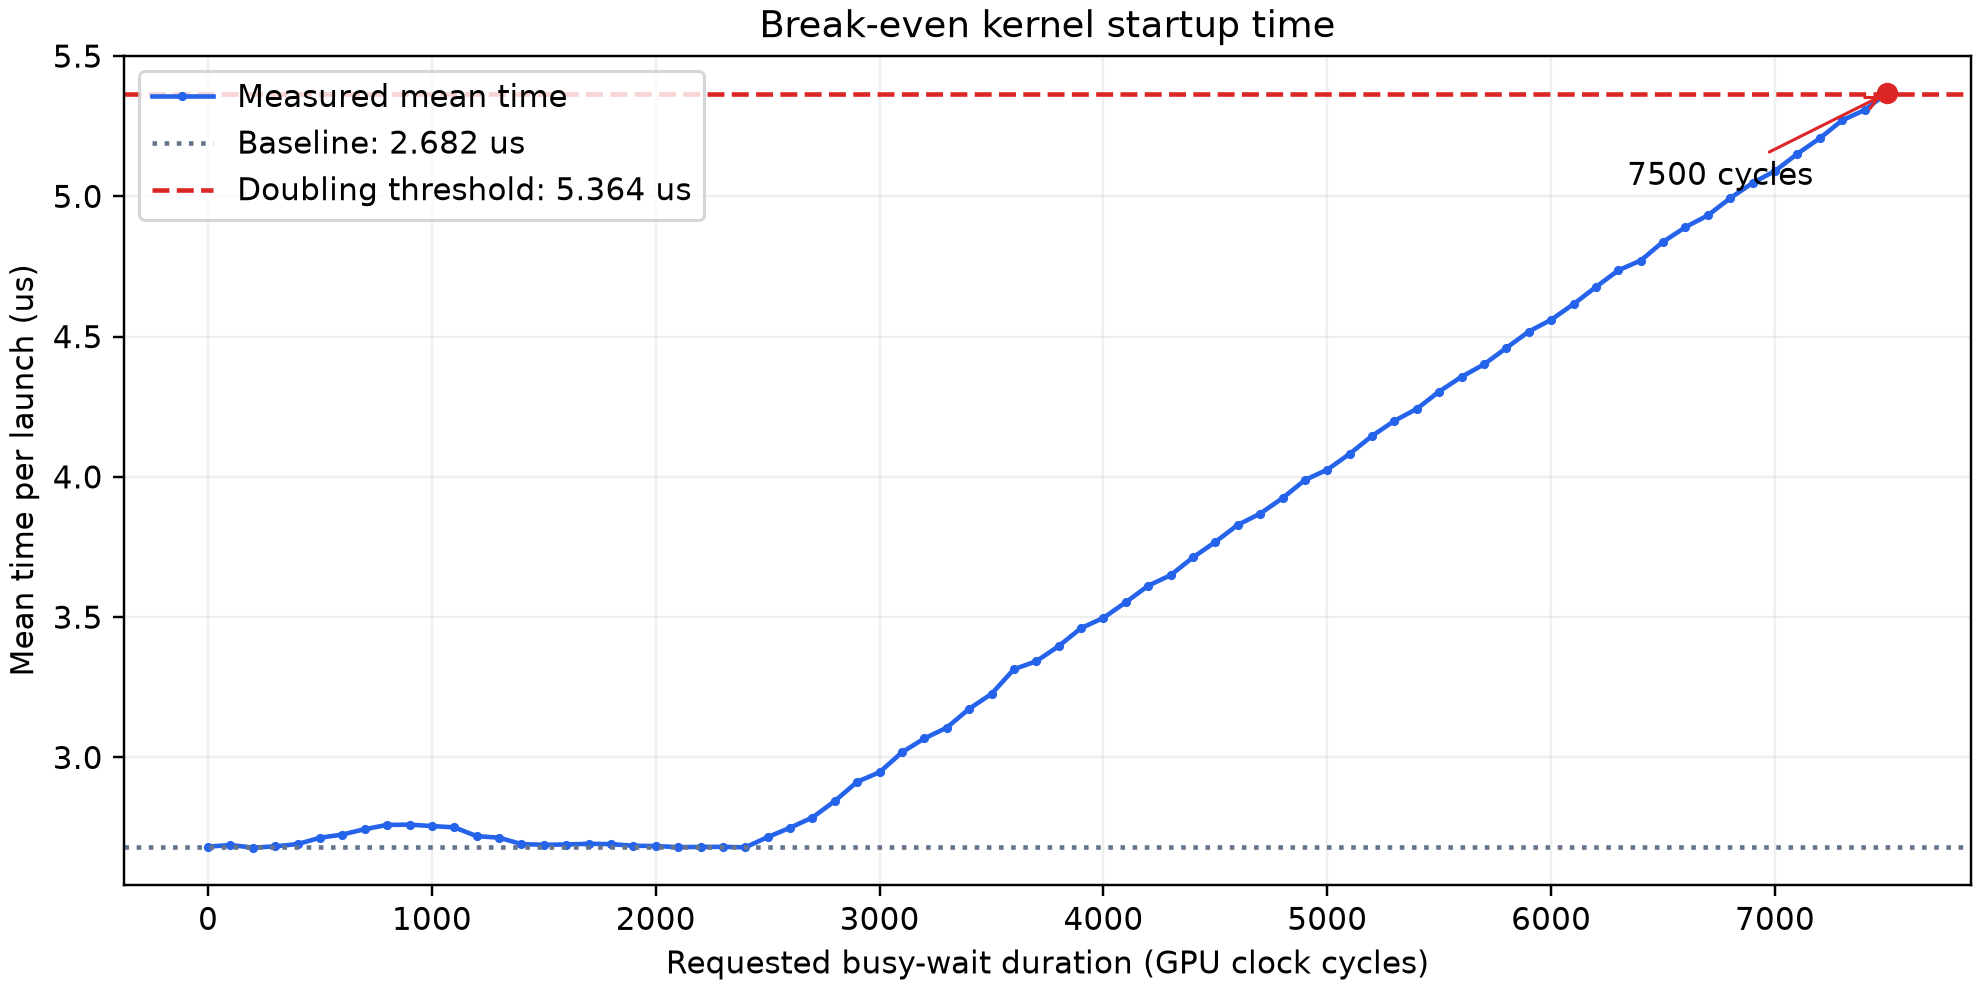
\includegraphics[width=0.91\linewidth]{break_even.png}
\caption{The 76 recorded points, including the zero-wait baseline. The first
point to reach the doubling threshold is at 7500 cycles.}
\label{fig:breakeven}
\end{figure}

\begin{center}
\begin{tabular}{@{}lr@{}}
\toprule
Quantity & Value \\
\midrule
Baseline \(T_0\) & \(2.681958\us\) \\
Threshold \(2T_0\) & \(5.363917\us\) \\
Mean at 7400 cycles & \(5.307372\us\) \\
Mean at 7500 cycles & \(5.367559\us\) \\
\bottomrule
\end{tabular}
\end{center}

Our measured break-even value is therefore \textbf{7500 GPU clock cycles}.
The 7400-cycle point is still below the threshold, and the next point is above
it. This locates the observed crossing within one 100-cycle search step.
Since the final point only just exceeds the threshold, another run could
shift the crossing slightly. We report the first crossing in this run,
without claiming a statistical uncertainty of 100 cycles.

\clearpage
\section*{2.3 PCIe Data Movements}

\subsection*{Setup and measurements}

We compared \code{cudaMemcpy()} transfers using pageable host memory from
\code{malloc()} and pinned host memory from \code{cudaMallocHost()}. We
tested both host-to-device (H2D) and device-to-host (D2H) copies. The results
in this section all come from job 279661 and its matching CSV file.

\begin{center}
\small
\begin{tabularx}{\linewidth}{@{}lX@{}}
\toprule
Parameter & Configuration \\
\midrule
GPU & NVIDIA GeForce RTX 2080 Ti \\
Host buffers & One pageable and one pinned buffer, each 1 GiB \\
Device buffer & One 1-GiB buffer allocated with \code{cudaMalloc()} \\
Transfer directions & H2D and D2H for both host-memory types \\
Recorded results & 44 measurements in \code{pcie\_results.csv} \\
\bottomrule
\end{tabularx}
\end{center}

We used 11 geometrically spaced transfer sizes:
\[
    S_k = 2^{10}\,4^k\ \text{bytes},\qquad k=0,\ldots,10.
\]
The first is 1 KiB and the last is 1 GiB. Testing four conditions at each size
gives \(11\times4=44\) measurements.

All buffers were allocated and initialized before timing. Each condition
began with three warm-up copies and a synchronization. We then timed a batch
of copies with \code{std::chrono::steady\_clock}, synchronized, and divided
the elapsed time by the number of copies. We used 1000 repetitions up to
64 KiB, 200 up to 1 MiB, 30 up to 16 MiB, 8 up to 256 MiB, and 4 at 1 GiB.

With the size \(S\) in bytes and the mean transfer time \(\overline{t}\) in
seconds, we calculated the bandwidth as
\[
    \mathrm{BW} = \frac{S}{10^9\,\overline{t}}\ \mathrm{GB/s}.
\]
Here GB/s uses decimal gigabytes, whereas KiB, MiB and GiB are binary units.
Allocation and initialization times are excluded.

The timer includes the copy calls and the final synchronization. This gives
the bandwidth seen by an application, rather than a measurement of bus
occupancy alone. The final synchronization matters for pageable H2D copies:
the API can return after staging the host data, before the transfer to the
device has finished.

The submitted Makefile uses \code{-O2} and \code{-std=c++14}. The exact CUDA
compiler and driver versions used for these jobs were not recorded.

\clearpage
\subsection*{Results}

\begin{figure}[!ht]
\centering
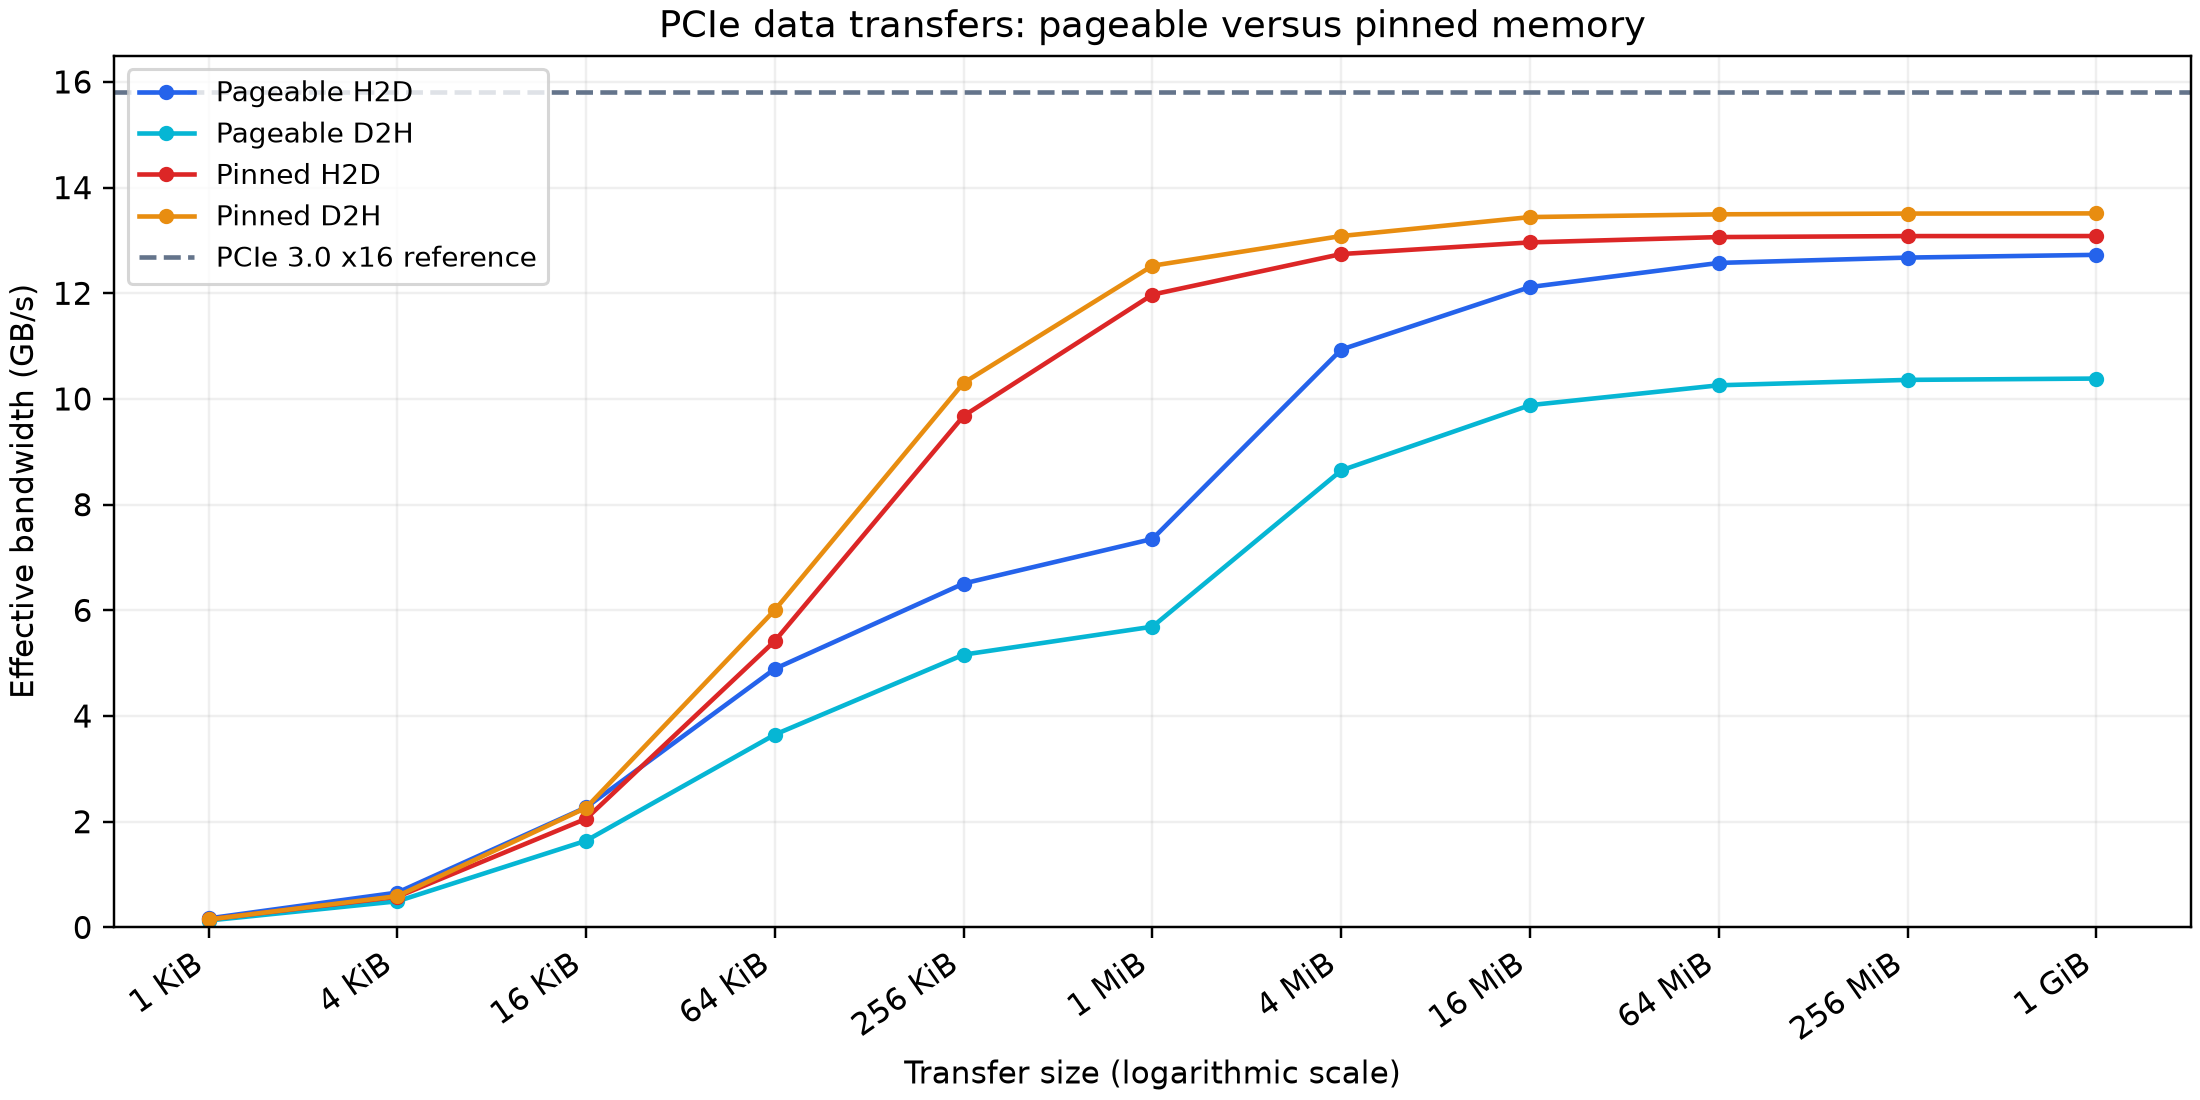
\includegraphics[width=\linewidth]{pcie_graph.png}
\caption{Effective transfer bandwidth for job 279661. Transfer size is shown
on a logarithmic axis. The dashed line is the assignment's theoretical
PCIe 3.0 x16 reference of \(15.8\,\mathrm{GB/s}\).}
\label{fig:pcie}
\end{figure}

\begin{table}[!ht]
\centering
\small
\begin{tabular}{@{}lrrrr@{}}
\toprule
Size & Pageable H2D & Pageable D2H & Pinned H2D & Pinned D2H \\
\midrule
1 KiB   & 0.1692  & 0.1294  & 0.1508  & 0.1492 \\
4 KiB   & 0.6585  & 0.4931  & 0.5783  & 0.5910 \\
16 KiB  & 2.2707  & 1.6400  & 2.0553  & 2.2631 \\
64 KiB  & 4.8941  & 3.6484  & 5.4209  & 6.0072 \\
256 KiB & 6.5075  & 5.1611  & 9.6800  & 10.3059 \\
1 MiB   & 7.3511  & 5.6906  & 11.9753 & 12.5216 \\
4 MiB   & 10.9348 & 8.6477  & 12.7425 & 13.0836 \\
16 MiB  & 12.1179 & 9.8830  & 12.9629 & 13.4422 \\
64 MiB  & 12.5747 & 10.2588 & 13.0637 & 13.4943 \\
256 MiB & 12.6756 & 10.3610 & 13.0824 & 13.5083 \\
1 GiB   & 12.7274 & 10.3862 & 13.0833 & 13.5118 \\
\bottomrule
\end{tabular}
\caption{Bandwidth in GB/s, rounded to four decimal places. The original CSV
contains the transfer times, bandwidths and repetition counts.}
\label{tab:pcie}
\end{table}

For small transfers, the cost of setting up a copy dominates. At 1 KiB, all
four cases achieve only about \(0.13\)--\(0.17\,\mathrm{GB/s}\). As the
transfer size grows, this fixed cost is spread over more bytes and the curves
level off. At 1 GiB, the measured range is
\(10.39\)--\(13.51\,\mathrm{GB/s}\). This is the practical reason to combine
small transfers when possible.

\clearpage
\subsection*{Pinned memory and transfer direction}

Pinned memory generally gives higher bandwidth for large transfers. At
1 GiB, H2D reaches \(13.0833\,\mathrm{GB/s}\) with pinned memory and
\(12.7274\,\mathrm{GB/s}\) with pageable memory, a gain of about \(2.8\%\).
For D2H, the corresponding values are \(13.5118\) and
\(10.3862\,\mathrm{GB/s}\), a gain of about \(30.1\%\). Pinned buffers
support direct DMA transfers, while pageable data may need an extra staging
step.

The two directions are not symmetric. Pageable H2D is faster than pageable
D2H at large sizes, whereas pinned D2H is slightly faster than pinned H2D.
Pinned memory also does not win in every case: at 1, 4 and 16 KiB, pinned H2D
is slower than pageable H2D. At these sizes, fixed overheads and timing
variation can outweigh the benefit of avoiding staging.

\subsection*{Comparison with the PCIe reference}

The highest measured bandwidth is \(13.5118\,\mathrm{GB/s}\), reached by
pinned D2H. Relative to the theoretical PCIe 3.0 x16 value in the exercise
sheet, this is
\[
    \frac{13.5118}{15.8}\times100\% \simeq 85.5\%.
\]
This is in the expected range once transfer overheads are included. We did
not independently check the negotiated PCIe generation and width, so
\(15.8\,\mathrm{GB/s}\) is used as the assignment's reference rather than
as a measured property of the link.

The results come from one selected execution. Repeating copies within a
condition reduces the effect of individual calls, but it does not tell us
how much a separate run would vary. CPU activity, caches and runtime behaviour
may affect the measured bandwidth, and the cost of allocating pinned memory
is outside this test.

Overall, the main pattern is clear: larger transfers use the available
bandwidth more effectively, and pinned memory gives the best large-transfer
performance. Its advantage is much larger for D2H than for H2D in this run.

\section*{2.4 Willingness to present}

Group 15 is willing to present all three exercises:
\begin{itemize}
    \item 2.1 Raw Kernel Startup Time;
    \item 2.2 Break-even Kernel Startup Time;
    \item 2.3 PCIe Data Movements.
\end{itemize}

\end{document}
